\chapter{Equipment Health Assessment using Artificial Neural Networks}%
\label{chapter:equipment_health_assessment_using_artificial_neural_networks}

\chapterintrobox{This chapter demonstrates the use of an artificial neural network to estimate the health state of a set of turbofan engines from NASA C-MAPSS dataset and predict the remaining useful life. Also different metrics to assess the performance of the network will be introduced.}

\section{Introduction to NASA C-MAPSS dataset}

C-MAPSS is a tool for simulating a realistic large commercial turbofan engine. The software is coded in the MATLAB\textsuperscript{\textregistered} and Simulink\textsuperscript{\textregistered} environment.

\begin{wrapfigure}{r}{0.5\textwidth}
    \centering
    \includegraphics[width=.48\textwidth]{figures/c-mapss-engine-diagram.jpg}
    \caption{Simplified diagram of engine simulated in C-MAPSS \cite{Saxena2008}}
    \label{figure:c-mapss-engine-diagram}    
\end{wrapfigure}

C-MAPSS software consists of many editable input parameters that controls the simulation, these inputs are specified by the user and control many aspects of the simulation such as operational profile, closed-loop controllers, environmental conditions, etc. \cite{Saxena2008}. 

Figure \ref{figure:c-mapss-engine-diagram} is a simplified diagram of the simulated engine showing its main elements, like low pressure compressor section (LPC), high pressure compressor section (HPC), fan and combustor. The dataset released by NASA Ames Research Center contains resulting data from simulating many turbofan engines, from beginning of operation until failure. The dataset was originally released for Prognostics and Health Management 2008 Data Competition, Table \ref{table:c-mapss-sensors} shows different variables, the output of the simulation and their units, that were provided for the participants in the competition:

\begin{table}[ht]
    \centering
    \begin{tabu}{lll}
		\tabucline[1.5pt]{-} 
        \textbf{Symbol} & \textbf{Description} & \textbf{Units}\\
        \hline
        \textbf{T2} & Total temperature at fan inlet & R \\
        \textbf{T24} & Total temperature at LPC outlet & R \\
        \textbf{T30} & Total temperature at HPC outlet & R  \\
        \textbf{T50} &Total temperature at LPT & R\\
        \textbf{P2} & Pressure at fan inlet& psia\\
        \textbf{P15}& Total pressure in bypass-duct& psia\\
        \textbf{P30}& Total pressure at HPC outlet& psia\\
        \textbf{Nf}& Physical fan speed& rpm\\
        \textbf{Nc} & Physical core speed &rpm\\
        \textbf{epr}& Engine pressure ratio (P50/P2)& --\\
        \textbf{Ps30}& Static pressure at HPC outlet& psia\\
        \textbf{phi}& Ratio of fuel flow to Ps30& pps/psi\\
        \textbf{NRf}& Corrected fan speed &rpm\\
        \textbf{NRc}& Corrected core speed& rpm\\
        \textbf{BPR}& Bypass Ratio& --\\
        \textbf{farB}& Burner fuel-air ratio &--\\
        \textbf{htBleed}& Bleed Enthalpy &-- \\
        \textbf{Nf\_dmd} &Demanded fan speed& rpm\\
        \textbf{PCNfR\_dmd}& Demanded corrected fan speed &rpm\\
        \textbf{W31} & HPT coolant bleed & lbm/s \\
        \textbf{W32} & LPT coolant bleed & lbm/ \\
		\tabucline[1.5pt]{-} 
    \end{tabu}
    \caption{C-MAPSS outputs to measure system response.}
    \label{table:c-mapss-sensors}
\end{table}

C-MAPSS data contains 4 datasets: FD001, FD002, FD003 and FD004. Each dataset has different working conditions and fault modes. Table \ref{table:c-mapss-statistics} contains statistics of the different datasets:

\begin{table}[ht]
    \centering
    \begin{tabu}{ccccc}
        
		\tabucline[1.5pt]{2-5} 
                    & units number  & max length    & average length    & min length    \\
       \hline
            FD001   & 100           & 362           & 206.31            & 128           \\
            FD002   & 260           & 378           & 206.77            & 128           \\
            FD003   & 100           & 525           & 247.2             & 145           \\
            FD004   & 249           & 543           & 245.95            & 128           \\
		\tabucline[1.5pt]{-} 
    \end{tabu}
    \caption{Units number and cycles length statistics in C-MAPSS data}
    \label{table:c-mapss-statistics}
\end{table}

\section{Visualization of equipment degredation}
Visualizing the simulation output can give a sense of how these variables change during the life of the engine, Figure \ref{fig:sensors-plot} shows four different sensors from one of the engines (values are normalized):

\begin{figure}[h]
    \centering
    \includegraphics[width=\linewidth]{figures/sensors_plot.pdf}
    \caption{Development of 6 sensors outputs from one of the engines (normalized)}
    \label{fig:sensors-plot}
\end{figure}
\begin{figure}[H]
    \centering
    \includegraphics[width=.9\linewidth]{figures/pca-degradation.pdf}
    \caption{Equipment health degredation (lighter colors indicate advancing of health degradation) of four turbofan engines from C-MAPSS dataset}
    \label{fig:pca-degradation}
\end{figure}

It is apparent that sensors output follow a specific pattern (increasing or decreasing) from beginning of operation until breakdown, this is very useful and can increase the robustness of the predictive model.

Alternatively, all sensors values can be combined and visualized altogether using Principal Component Analysis (section \ref{section:dimensionality-reduction}) to reveal the general trend in the datat, if condition monitoring data is directly indicative of the equipment health state, visualization of principal components can show apparent visual degradation patterns.

Sensors values from 4 different engines are combined using PCA and the two first principal components are represented on Figure \ref{fig:pca-degradation}. 

There is absolutely an apparent pattern for health state degradation across the different engines from left (where darker colors indicate normal working state) to the right (where the lighter colors indicate fault development).

\section{Engines health classification}
Before proceeding with a complicated task such as \acrshort{rul} estimation, a simpler task like engines health classification can show the complexity of the problem. This section describes using neural networks to classify engines states as healty or faulty. The first and last 25 cycles from each unit are considered to be healthy and faulty respectively.

A neural network that uses all 24 inputs (all operational settings and sensors) with two hidden layers is used to carry out this classification. Table \ref{table:c-mapss-classifier-architecture} summarizes the network architecture:

\begin{table}[ht]
    \centering
    \begin{tabu}{lll}
		\tabucline[1.5pt]{-}
		\textbf{Layer (type)}   & \textbf{Output shape} &   \textbf{Param \#} \\
		\tabucline[1pt]{-}
		Dense1 (Dense) 			&   (None, 8)   &   200\\
		Dense2 (Dense) 	        &   (None, 4)   &   36       \\
		Dense3 (Dense)			&   (None, 1)   &   5   \\
		\tabucline[1pt]{-}
		Total params: 241       &                   &           \\
		Trainable params: 241   &                   &           \\
		Non-trainable params: 0     &                   &           \\
	\tabucline[1.5pt]{-}
    \end{tabu}
    \caption{C-MAPSS classifier architecture}
    \label{table:c-mapss-classifier-architecture}
\end{table}

The model is trained for 200 epochs with batch size of 32 samples, the classifier achieves \textbf{93.46\% accuracy} on the test set. Figure \ref{fig:cmapss-classifier-training} shows the training process of the network. In the upper plot, the y-axis corresponds to the train and validation losses (binary crossentropy). The y-axis in the lower plot corresponds to the network train and validation accuracies, the x-axis shared between the two plots indicates the training epochs. Although the validation accuracy varies a lot, the training accuracy keeps improving with each epoch.

\begin{figure}[H]
    \centering
    \includegraphics{figures/cmapss_classification_training.pdf}
    \caption{Training process of C-MAPSS classifier}
    \label{fig:cmapss-classifier-training}
\end{figure}

Figure \ref{fig:cmapss-classifier-roc} shows \acrlong{roc} (\acrshort{roc}) Curve of the classifier with a high \acrlong{auc} (\acrshort{auc}). Other classification metrics are shown in Table \ref{table:cmapss-classifier-metrics}.

\begin{figure}[H]
    \centering
    \includegraphics{figures/cmapss_classification_roc.pdf}
    \caption{C-MAPSS classifier ROC curve on test set}
    \label{fig:cmapss-classifier-roc}
\end{figure}

\begin{table}[H]
    \centering
    \begin{tabu}{cccccc}
        
    \tabucline[1.5pt]{-}
    \textbf{Metric} &  \textbf{Exactitude} &  \textbf{Précision} &  \textbf{Recall} &  \textbf{F-1} &  \textbf{ROC AUC}  \\
    \hline
    \textbf{Score} & 93.43\% & 0.90 & 0.98 & 0.94 & 0.9332 \\
	\tabucline[1.5pt]{-}
    \end{tabu}
    \caption{C-MAPSS classifier metrics on test set}
    \label{table:cmapss-classifier-metrics}
\end{table}

\section{Remaining Useful Life prediction}
\subsection{Remaining Useful Life modeling}
In order to train a neural network to estimate the \acrlong{rul} (\acrshort{rul}) of a new unseen data from C-MAPSS dataset, an appropriate \acrshort{rul} that corresponds to the training data must be constructed. \acrshort{rul} was defined in Section \ref{section:rul}, from this definition several approaches to construct an appropriate \acrshort{rul} can be developed for units in the train data (where the total number of cycles before failure is known). The simplest approach is to use an always-decreasing \acrshort{rul}, this implies that the equipment state is always decreasing and moving towards failure. The problem with this approach is that degradation process isn't linear and in real life, machines don't start to degrade as soon as they are start working. A second approach is to use a piecewise function where the equipment state is constant at first then at a specific point it starts to degrade linearly. This approach is much better than the first one but it is not very representative of the real world behaviour of degradation process. In the context of this thesis, \acrshort{rul} is approached as a nonlinear polynomial function where the degradation is slow at first then accelerates towards the end of life. Figure \ref{fig:rul-models} shows the different choices for modeling \acrshort{rul}:

\begin{figure}[H]
    \centering
    \includegraphics{figures/rul_models.pdf}
    \caption{Different \acrshort{rul} modeling choices}
    \label{fig:rul-models}
\end{figure}

It must be noted that not any of these approaches can be claimed to be representative of the real world degradation process, but choosing the most intuitive representation of \acrshort{rul} can help the learning algorithm learn the implicit degradation trends in the data.

\subsection{\acrshort{rul} prediction using feed-forward network}
The last section dealt with classifying units health state as healthy or faulty. This section instead presents a neural network for estimating the \acrshort{rul}. In this section, a neural network architecture with 3 hidden layers is used. Since this is a regression problem, mean squared error is used as the loss function, mean absolute error is used as a metric for the model. Table \ref{table:cmapss-regression-architecture} presents the architecture details:

\begin{table}[h]
    \centering
    \begin{tabu}{lll}
		\tabucline[1.5pt]{-}
		\textbf{Layer (type)}   & \textbf{Output shape} &   \textbf{Param \#} \\
		\tabucline[1pt]{-}
		Dense1 (Dense) 			&   (None, 32)  &       800     \\
		Dense2 (Dense)          &   (None, 16)  &       528     \\
		Dense3 (Dense)          &   (None, 8)   &       136     \\
		Dense4 (Dense)          &   (None, 1)   &       9       \\

		\tabucline[1pt]{-}
		Total params: 1,473       &                   &           \\
		Trainable params: 1,473   &                   &           \\
		Non-trainable params: 0   &                   &           \\
	\tabucline[1.5pt]{-}
    \end{tabu}
    \caption{Fully-connected network architecture for \acrshort{rul} prediction}
    \label{table:cmapss-regression-architecture}
\end{table}

The network was trained for 300 epochs, batch size of 128 samples. Figure \ref{fig:cmapss-regression-training} shows the training process of the network. The figures show the development of training and validation losses (mean squared error) and metrics (mean absolute error) respectively as a function of training epochs.

\begin{figure}[H]
    \centering
    \includegraphics{figures/cmapss_regression_training.pdf}
    \caption{Training process of \acrshort{rul} predictor}
    \label{fig:cmapss-regression-training}
\end{figure}

After training, the model is evaluated on two units from the test set. Figure \ref{fig:cmapss-regression-prediction} shows the actual \acrshort{rul} (dashed line), model prediction at each cycle and a 3rd degree polyomial fit of model's predictions.

\begin{figure}[H]
    \centering
    \includegraphics{figures/cmapss_regression_predictions.pdf}
    \caption{Prediction results on two test units}
    \label{fig:cmapss-regression-prediction}
\end{figure}

Although the model's prediction are close the the actual \acrshort{rul}, but they are noisy and there is so much fluctuation. The noise can be reduced by smoothing the output for example using moving average or fitting the points to a polynomial. But the reason of the noise in the first place is that fully-connected architecture doesn't take into consideration the previous predictions (i.e. acyclic architecture). Since \acrshort{rul} at each instant of time depends on the \acrshort{rul} from the previous one, taking previous steps into consideration while making new predictions can effectively reduce the noise and also improve prediction accuracy. To achieve that, a cyclic neural archtiecture like recurrent neural networks should be used.

\subsection{Improving \acrshort{rul} prediction using LSTM networks}
Fully-connected neural networks are powerful tool for modeling a wide range of problems, but using the fully-connected architecture for time series prediction, such as \acrshort{rul} prediction, can yield very noisy output because the network is acyclic and each instant in time is evaluated seperately and doesn't take into account the previous predictions. \acrlong{lstm} (Section \ref{section:lstm}) are a powerful tool for modeling such problems and to make more robust and less noisy predictions. In this section, fully-connected neural network architecture from previous section is replaced with an \acrshort{lstm} network to predict \acrshort{rul} in C-MAPSS dataset.

The architecure used here is described in Table \ref{table:cmapss-lstm-architecture}:

\begin{table}[h]
    \centering
    \begin{tabu}{lll}
		\tabucline[1.5pt]{-}
		\textbf{Layer (type)}   & \textbf{Output shape} &   \textbf{Param \#} \\
		\tabucline[1pt]{-}
		LSTM1 (LSTM) 			&   (None, 100, 100)    &       50000   \\
		LSTM2 (LSTM)           &   (None, 100, 100)    &       80400   \\
		LSTM3 (LSTM)           &   (None, 75)          &       52800   \\
        Dense1 (Dense)         &   (None, 120)         &       9120    \\
        Dense2 (Dense)         &   (None, 110)         &       13310   \\
        Dense3 (Dense)         &   (None, 100)         &       11100   \\
		\tabucline[1pt]{-}
		Total params: 216,730       &                   &               \\
		Trainable params: 216,730   &                   &               \\
		Non-trainable params: 0     &                   &               \\
	\tabucline[1.5pt]{-}
    \end{tabu}
    \caption{LSTM network architecture for \acrshort{rul} prediction}
    \label{table:cmapss-lstm-architecture}
\end{table}

It is apparent that the \acrshort{lstm} architecture has much more parameters (216,730 parameters) than fully-connected architecture (1,473). This is because of the more complicated design of \acrshort{lstm} cells and their possession of different gates. This results in much longer training time.

\acrshort{lstm} layers take 3 dimensional tensor as an input of shape \textit{(samples, sequence length, features)}. Sequence length was set to 100 in this architecture, that's why every training sample must have a shape of \textit{(sequence length, features)}. All units have the same number of features but different legnths, since every sample must have a sequence length of 100, samples with cycles less than 100 are padded with -10 where \acrshort{lstm} layers are set to ignore any time steps with this value.

The network was trained for 50 epochs with batch size of 16 and validation split of 0.2 using Adam optimizer. Training process is visualized in Figure \ref{fig:cmapss-lstm-training}:

\begin{figure}[H]
    \centering
    \includegraphics{figures/cmapss_lstm_training.pdf}
    \caption{LSTM training process}
    \label{fig:cmapss-lstm-training}
\end{figure}

Table \ref{table:cmapss-lstm-results} shows the loss and metric (i.e. mean absolute error) on the different train, validation and test sets:

\begin{table}[H]
	\centering
	\begin{tabu}{lcc}
		\tabucline[1.5pt]{2-3} 
						&	\textbf{Loss}	&	\textbf{Mean Absolute Error}	\\
	   \tabucline[1pt]{-}
		Train set 		&	1600.60			    &	25.43				\\
		Validation set 	&	3039.68 			&	36.37					\\
		Test set		&	1379.67 			&	23.27					\\
   \tabucline[1.5pt]{-}
   \end{tabu}
   \caption{\acrshort{lstm} training results}
   \label{table:cmapss-lstm-results}
\end{table}

Four different units were reserved as testing units, after training the network is used to predict \acrshort{rul} on test units. Figure \ref{fig:cmapss-lstm-prediction} shows prediction results and actual \acrshort{rul} of two different units.

\begin{figure}[h]
    \centering
    \includegraphics{figures/cmapss_lstm_regression_predictions.pdf}
    \caption{LSTM prediction results on two test units}
    \label{fig:cmapss-lstm-prediction}
\end{figure}

It's apparent that \acrshort{lstm} network predictions are much better and almost free of noise compared to those made by the fully-connected network shown in Figure \ref{fig:cmapss-regression-prediction}. Predicted \acrshort{rul} is almost identical to actual \acrshort{rul} towards the end of life of the unit.


\section{Application to oilfield equipment}%
\label{sec:application_to_oilfield_equipment_1}
This chapter presented a predictive maintenance approach for \acrshort{rul} estimation based on condition monitoring data provided by different sensors that can measure different physical variables that are related to the equipment's health state. The data used in the previous sections consisted of C-MAPSS turbofan engines dataset, but the same approach can be extended to other applications like oil rigs.

Modern oil rigs contain a large number of sensors distributed across almost every critical equipment. These sensors measure different physical variables such as temperature, flow, pressure…. But the majority of the data provided by these sensors isn't properly exploited into an appropriate framework of prognostics and predictive maintenance, there are enormous amounts of historic data in oil rigs that if exploited can greatly enhance maintenance programs in such critical applications where reducing downtime is very important and equipment unavailability can have cause significant production losses.

\begin{figure}[p!]
	\centering
	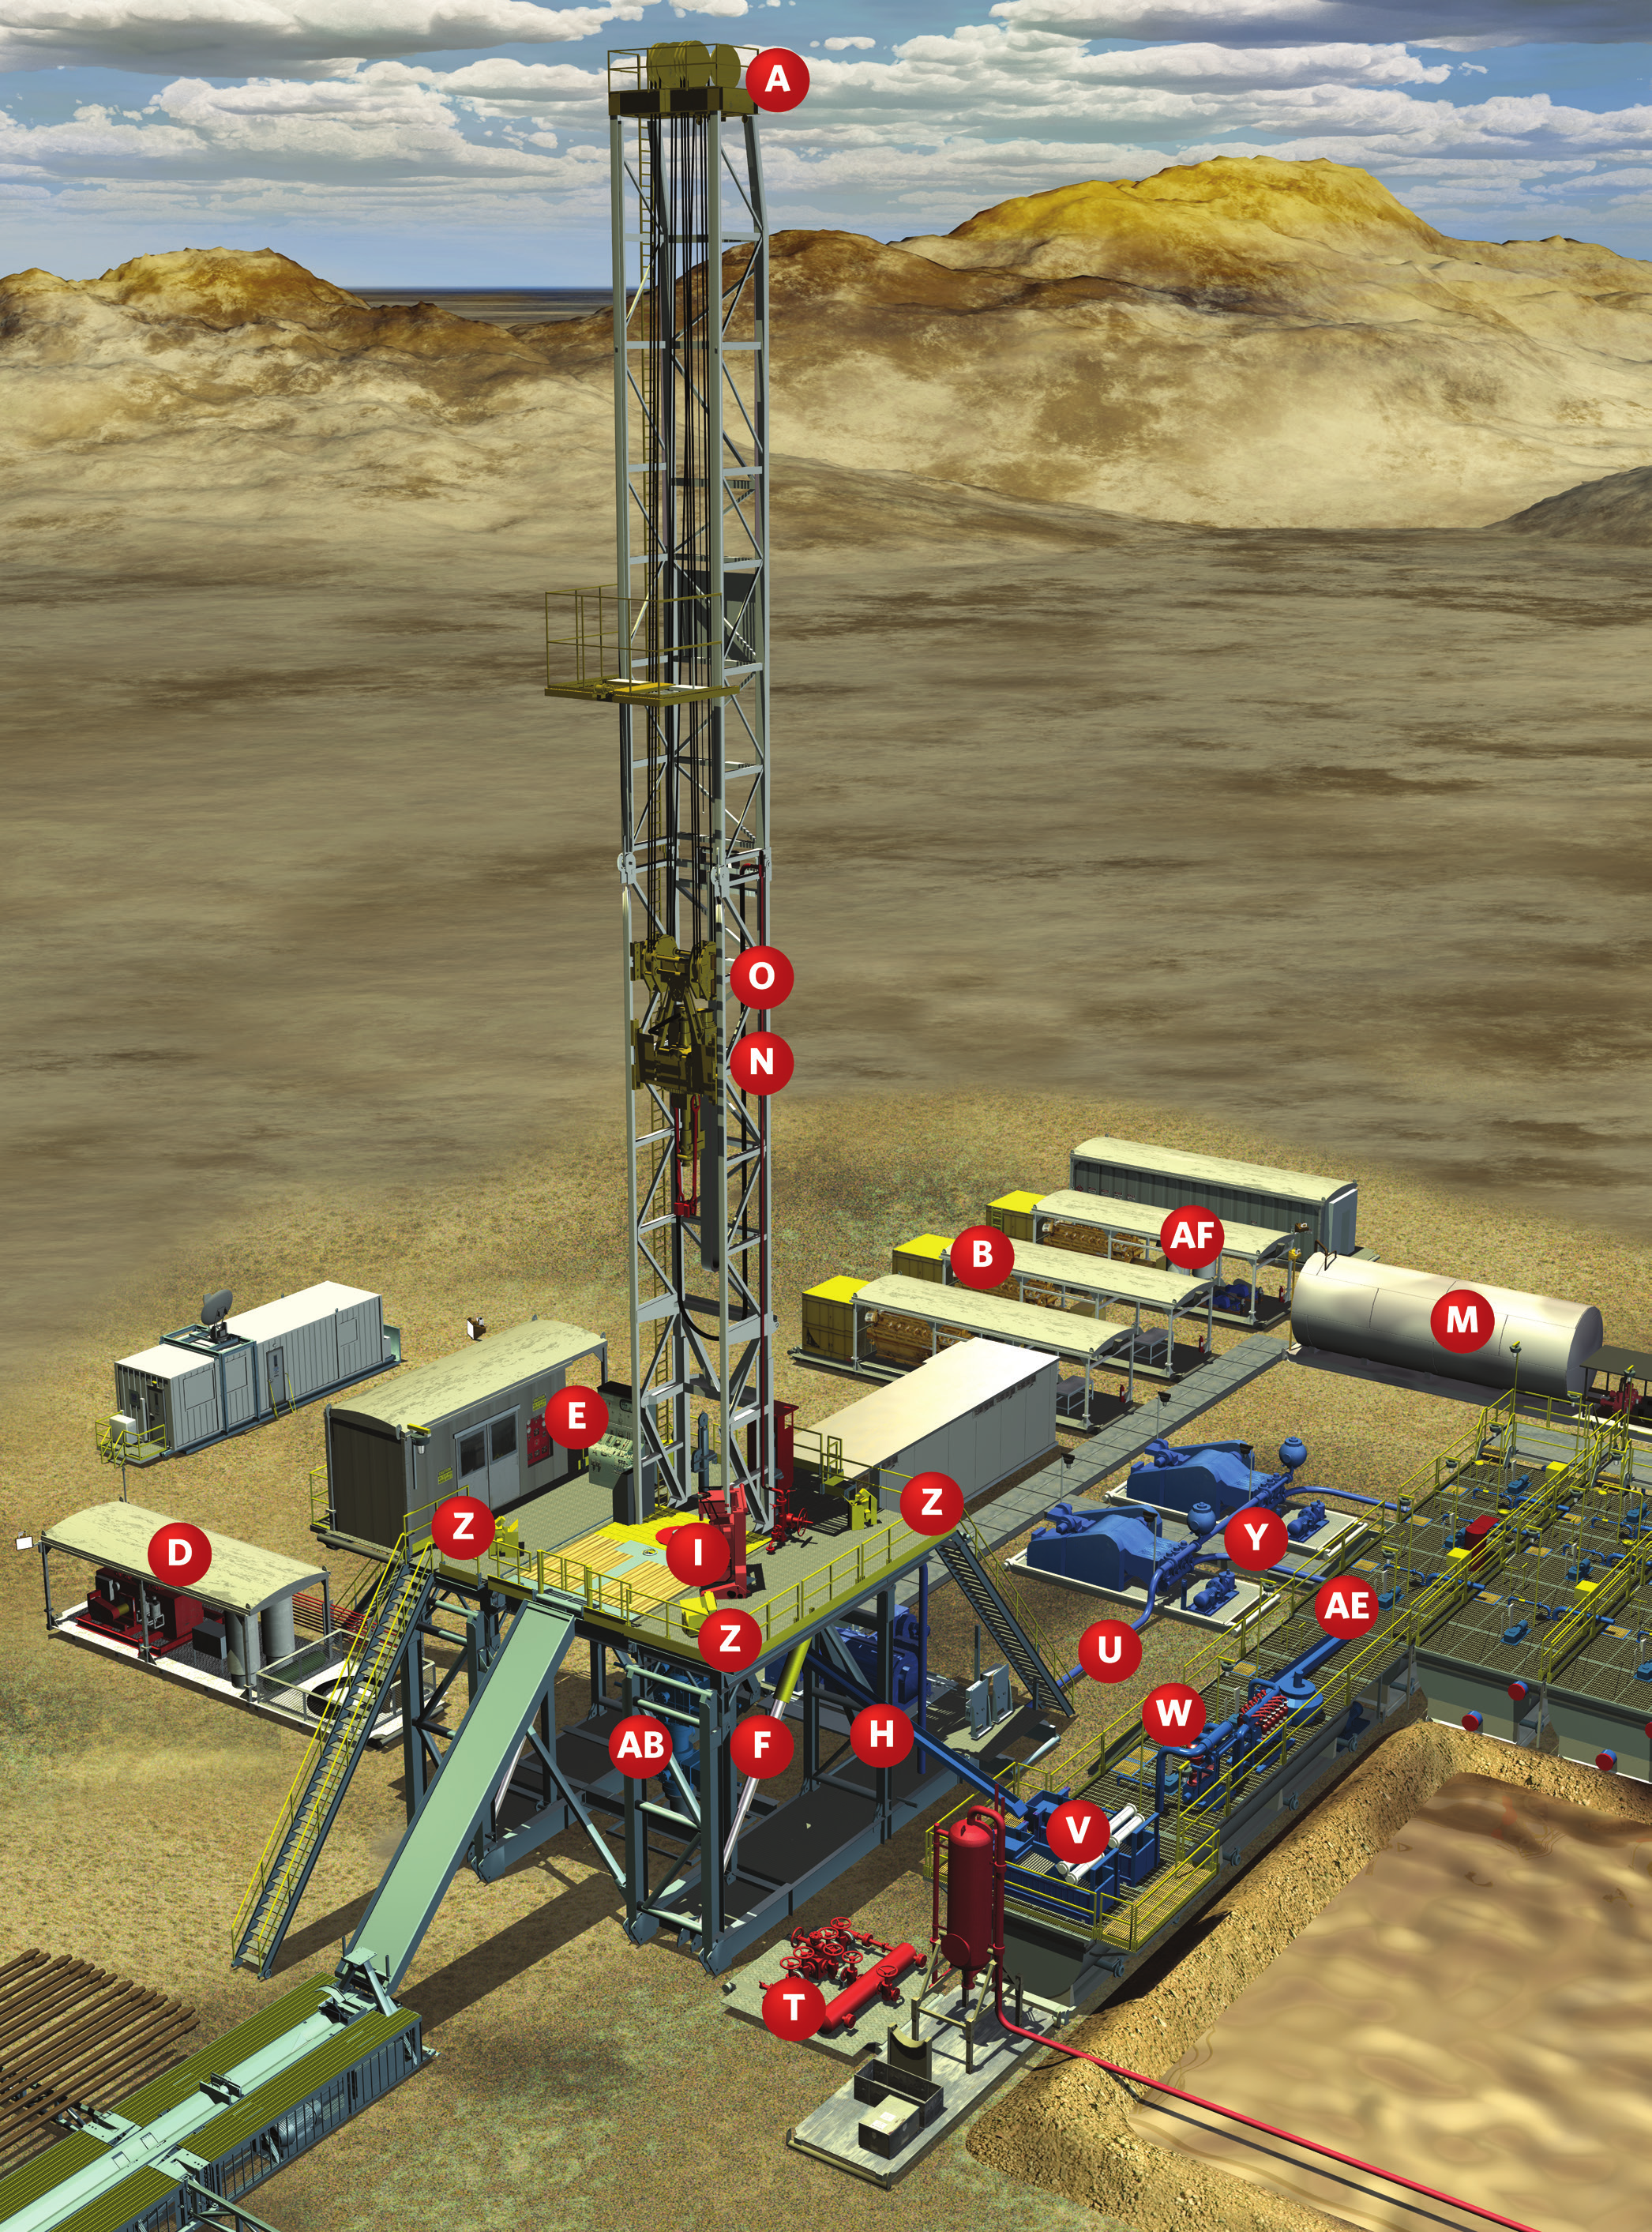
\includegraphics[width=0.9\linewidth]{figures/honeywell-oilrig-sensors.png}
	\caption{List of sensors installed on oil rigs for monitoring}%
	\label{fig:honeywell-oilrig-sensors}
\end{figure}

Figure \ref{fig:honeywell-oilrig-sensors} shows different spots where sensors are installed on most modern oil rigs. Table \ref{table:honeywell-oilrig-sensors} lists types of different sensors that can be used for prognostics, the units to which they are attached and which physical variables they can measure. A neural network can be trained on the rig historic data and be used to monitor different equipments, their interaction, detect anomalies and report them in time in order to carry on the appropriate maintenance actions.

\begin{table}[p!]
	\centering
	\begin{adjustbox}{angle=90}
	\begin{tabu}{clp{30mm}p{120mm}}
		\tabucline[1.5pt]{-} 
		\textbf{Sensor} & \textbf{Equipment} & \textbf{Sensor Type}  & \textbf{Measured quantity}\\
        \hline
A&	Crown Block &	Load cell	&	Weight on drill line via cable tension\\
B& Power Generation Unit	&	Pressure&	Oil, water, and hydraulic fluid pressure\\
D&Accumulator Unit	&	Pressure&	Inlet/outlet pressure with high accuracy\\
F&Rig Hydraulic Lift	&	Pressure&	Hydraulic pressure, weight, force/strain, or movement, monitor raising or lowering deck for directional drilling\\
H&Drawworks	&	Load cells	&	Torque, load/weight/position while guiding pipe into position\\
M&Water/Storage Tank	&	Pressure& Tank liquid levels\\
N&Top Drive	&	Torque/Pressure&	Monitor torque/twisting movement to ensure right amount of force is applied. Weight on drill bit. Hydraulic pressure and feed information into control system.\\
O&Trabeling Block	&	Load cells	&	Weight on the drill line via cable tension\\
R&Deadline anchor	&	Load cells	&	Tension on deadline/drilling line cable\\
U&Mud Return Line	&	Pressure&	Drilling mud pressure to monitor and control mud flow\\
Y&Mud Pump	&	Pressure&	Pressure and flow of mud media\\
AB&BlowOut Preventor &	Pressure&	Monitor RAM position via hydraulic volumetric or pressure behind the piston\\
AD&Drill Bit	&	Pressure&	Pressure or differential pressure at high temperature and pressure ranges\\
AE	&	Fluid manifold	&	Pressure	&	Drilling fluid pressure\\
AF&Mud Tank/Reservoir	&	Pressure&	Tank liquid levels\\
		\tabucline[1.5pt]{-} 
    \end{tabu}
\end{adjustbox}
    \caption{Honeywell oilrig sensors list}
    \label{table:honeywell-oilrig-sensors}

\end{table}



\section{Conclusion}
Fully-connected neural networks are a powerful tool for quantifying health state of complex systems using condition monitoring data. C-MAPSS dataset is an example of a system with many interacting parts that provide a variety of condition-monitoring data (e.g. temperature, pressure, rpm, …) where the degradation isn't directly related to one component but is indicated by the sum of the trends in all the monitoring data. Neural networks are able to capture such trends and predict the \acrshort{rul} of the system before failure. Fully-connected networks were first used for this task, but a cyclic architecture like \acrshort{lstm} can produce better results with improved accuracy and much less noise.
